\newcommand{\gam}{\gamma}
\newcommand{\chio}{\chi_0}
\newcommand{\chior}{\chio(r)}
\newcommand{\Gam}{\Gamma}
\newcommand{\drp}{\dd{r'}}
\newcommand{\En}{E_n}
\newcommand{\kn}{k_n}

\newcommand{\hql}{h_l^{(1)}\!}
\newcommand{\ks}{k^*}
\newcommand{\sigtot}{\sig_\text{tot}}

\begin{statement}{}
	Consider a three dimensional potential
	\beq
		V(r) = \frac{\hbar^2 \gam}{2m} \del(r - a).
	\eeq
	The $s$ wave {\Schrodinger} equation is given by
	\beq
		-\frac{\hbar^2}{2m} \dv[2]{\chior}{r} + \frac{\hbar^2 \gam}{2m} \del(r - a) \, \chior = E \,\chior.
	\eeq
	The $s$ wave function must be regular (zero) at $r = 0$.  At $r = a$, it is continuous, but its derivative can jump.
\end{statement}

\begin{problem}
	Calculate the $s$ wave scattering phase shift $\delo(k)$, where $k$ is related to $E$ as $E = \hbar^2 k^2 / 2m$.
\end{problem}

\begin{solution}
	Sakurai (7.7.2) gives the integral equation for the partial wave,
	\beqn \label{delint}
		\frac{e^{i \dell} \sin\dell}{k} = -\frac{2m}{\hbar^2} \intoi \jl(kr) \, V(r) \, \Al(k; r) \, r^2 \dr.
	\eeqn
	This is given in the statement of Problem 8.b in Sakurai, as is
	\beqn \label{radint}
		\Al(r) = \jl(kr) - \frac{2 i m k}{\hbar^2} \intoi \jl(k r_<) \, \hql(k r_>) \, V(r') \, \Al(k; r') \, {r'}^2 \drp,
	\eeqn
	where $\hql$ are the spherical Hankel functions, defined by (A.5.18),
	\beqn \label{hankel}
		\hql(\rho) = \jl(\rho) + i \nl(\rho),
	\eeqn
	where $r_<$ is the smaller of $r$ and $r'$, and $r_>$ the larger.  Also, $\nl$ are the spherical Neumann functions, given by (A.5.12),
	\beq
		\nl(\rho) = (-1)^{l+1} \sqrt{\frac{\pi}{2\rho}} J_{-l-1/2}(\rho).
	\eeq
	
	For $r < a$, \refeq{radint} becomes
	\beq
		\Al(k; r) = \jl(kr) - \frac{2 i m k}{\hbar^2} \intoi \jl(kr) \, \hql(kr') \, \frac{\hbar^2 \gam}{2m} \del(r' - a) \, \Al(k; r') \, {r'}^2 \drp
		= \jl(kr) - i k a^2 \gam \jl(kr) \, \hql(ka) \, \Al(k; a),
	\eeq
	and for $r > a$,
	\beq
		\Al(k; r) = \jl(kr) - \frac{2 i m k}{\hbar^2} \intoi \jl(kr') \, \hql(kr) \, \frac{\hbar^2 \gam}{2m} \del(r' - a) \, \Al(k; r') \, {r'}^2 \drp
		= \jl(kr) - i k a^2 \gam \jl(ka) \, \hql(kr) \, \Al(k; a).
	\eeq
	At $r = a$, both equations become
	\beq
		\Al(k; a) = \jl(ka) - i k a^2 \gam \hql(ka) \, \jl(ka) \, \Al(k; a)
		\qimplies
		\Al(k; a) = \frac{\jl(ka)}{1 + i k a^2 \gam \, \jl(ka) \, \hql(ka)}.
	\eeq
	
	Using this result, \refeq{delint} gives us
	\beq
		\frac{e^{i \dell} \sin\dell}{k} = -\frac{2m}{\hbar^2} \intoi \jl(kr) \, \frac{\hbar^2 \gam}{2m} \del(r - a) \, \Al(k; r) \, r^2 \dr
		= -a^2 \gam \, \jl(ka) \, \Al(k; a)
		= -\frac{a^2 \gam \, \jl^2(ka)}{1 + i k a^2 \gam \, \jl(ka) \, \hql(ka)},
	\eeq
	or
	\beqn \label{sindelo}
		e^{i \dell} \sin\dell = -\frac{k a^2 \gam \, \jl^2(ka)}{1 + i k a^2 \gam \, \jl(ka) \, \hql(ka)}.
	\eeqn
	From \refeq{hankel}, according to Gottfried Ch.~15~(5) we can write
	\beq
		\tan\dell = -\frac{k a^2 \gam \, \jl^2(ka)}{1 - k a^2 \gam \, \jl(ka) \, \nl(ka)}.
	\eeq
	
	For the $s$ wave, the relevant $\jo$ is given by \refeq{jo}, and from (A.5.12),
	\beqn \label{no}
		\no(\rho) = -\frac{\cos\rho}{\rho}.
	\eeqn
	Then
	\beqn \label{tandelo}
		\tan\delo = -\frac{k a^2 \gam \, \jo^2(ka)}{1 - k a^2 \gam \, \jo(ka) \, \no(ka)}
		= -\frac{k a^2 \gam \, \sin^2 ka / (ka)^2}{1 + k a^2 \gam \sin ka \cos ka / (ka)^2}
		= -\frac{\gam \, \sin^2 ka}{k + \gam \sin ka \cos ka}
	\eeqn
	and so we have found
	\beqn \label{delo}
		\delo(k) = \tan^{-1}\!\!\left( -\frac{\gam \, \sin^2 ka}{k + \gam \sin ka \cos ka} \right).
	\eeqn
	\vfix
\end{solution}



\begin{problem}
	When $\gam \gg k$, $1/a$ and when $\sin ka$ is not small, discuss the behavior of the scattering phase shift.
\end{problem}

\begin{solution}
	In the limit $\gam \gg k$, \refeq{delo} becomes
	\beq
		\delo \to \tan^{-1}\!\!\left( -\frac{\gam \, \sin^2 ka}{\gam \sin ka \cos ka} \right)
		= \tan^{-1}\!\left[ -\cot ka \right]
		= \tan^{-1}\!\left[ \cot(-ka) \right]
		= -ka.
	\eeq
	This is the same as the hard sphere result discussed in Sec.~7.6 of Sakurai and given in (7.6.44).  When the delta function potential's strength $\gam$ becomes very large compared to the energy $E = \hbar^2 k^2 / 2m$ of an incoming particle (coming from outside), the particle will not be able to penetrate the shell.  This physical situation is just like the particle scattering off the surface of an infinitely hard sphere, so it makes sense that the phase shift is the same in both situations.
\end{solution}



\begin{problem}
	Obtain the condition to have resonant states and calculate the energy of the resonant states.
\end{problem}

\begin{solution}
	From the discussion in Sec.~7.8 of Sakurai, at a resonance where $k = \ks$ we must have
	\begin{align} \label{conds}
		\cot[\dell(\ks)] &= 0, &
		\left. \dv{\cot\dell}{k} \right|_{\ks} < 0.
	\end{align}
	From \refeq{tandelo},
	\beq
		\cot\delo = -\frac{k + \gam \sin ka \cos ka}{\gam \, \sin^2 ka} = 0
		\qimplies
		-\frac{k}{\gam} = \sin ka \cos ka = \frac{\sin(2ka)}{2}.
	\eeq
	Rearranging this, we obtain
	\beqn \label{thingy}
		\sin(2ka) = -\frac{2ka}{\gam a},
	\eeqn
	which we may solve graphically.  As shown in Fig.~\ref{plot3}, \refeq{thingy} has roots near $ka = n \pi / 2$ for $n = 0, 1, 2, \ldots \lessapprox 2\gam$.  As $\gamma$ increases, they become closer to $n\pi$.
	
	\begin{figure} \centering
		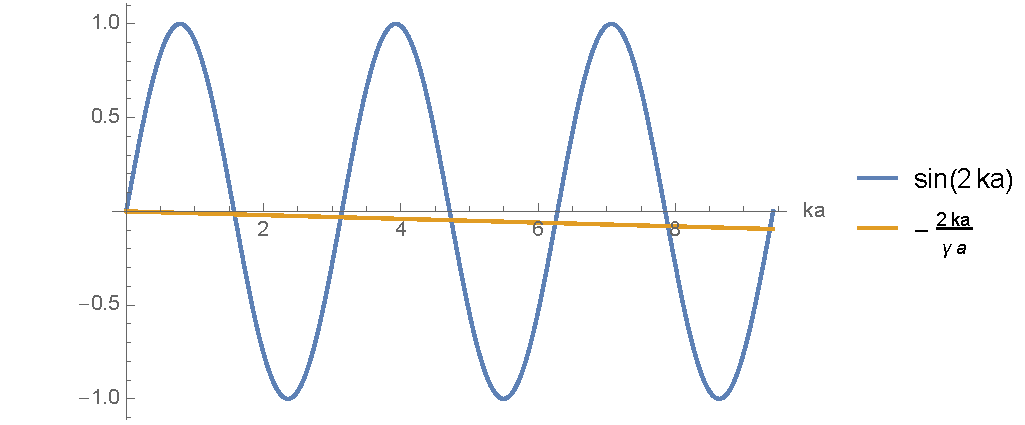
\includegraphics[width=0.75\textwidth]{plot3}
		\caption{Plot demonstrating roots of \refeq{thingy}.  The roots at $n \pi$ ($n = 0, 1, 2, \ldots$) correspond to resonances.}
		\label{plot3}
	\end{figure}
	
	We must determine which roots fulfill the second condition in \refeq{conds}.  Note that
	\begin{align}
		\dv{\cot\delo}{k} &= -\dv{k} \left( \frac{k}{\gam} \csc^2 ka + \cot ka \right)
		= -\left[ \frac{\csc^2 ka}{\gam} \dv{k}{k} + \frac{k}{\gam} \dv{k} \bigg( \csc^2 ka \bigg) + \dv{k} \bigg( \cot ka \bigg) \right] \notag \\
		&=  -\frac{\csc^2 ka}{\gam} + \frac{2 ka}{\gam} \cot ka \csc^2 ka + a \csc^2 ka
		= \frac{a\gam - 1 + 2 ka \cot ka}{\gam \sin^2 ka}. \label{delder}
	\end{align}
	For $\ks = n\pi/2$ with $n$ odd,
	\beq
		\left. \dv{\cot\delo}{k} \right|_{\ks} = \frac{a \gam - 1}{\gam} \sim a \not< 0,
	\eeq
	since \refeq{thingy} has no solutions if $a \gam < 1$.  For $n$ even, applying L'Hospital's rule gives us
	\beq
		\lim_{k \to \ks} \dv{\cot\delo}{k} = \lim_{k \to \ks} \frac{\cot ka - ka \csc^2 ka}{\gam \sin ka \cos ka} = -\infty,
	\eeq
	since $\csc^2 ka$ blows up faster than $\cot ka$.  So we have $ka \approx n\pi$ for $n = 0, 1, 2, ... \lessapprox \gam$.
	
	In the limit $\gam \gg k$, we may approximate the offset of the resonances from the $x$ as $-1 / \gam a$.  Then the condition for resonance is
	\beq
		\kn \approx \frac{n \pi}{a} \left( 1 - \frac{1}{\gam a} \right), \quad n = 0, 1, 2, ... \lessapprox \gam,
	\eeq
	and the energies of the resonant states are
	\beq
		\En \approx \frac{n^2 \pi^2 \hbar^2}{2 m a^2} \left( 1 - \frac{2}{\gam R} \right), \quad n = 0, 1, 2, ... \lessapprox \gam,
	\eeq
	where we have dropped terms of $\order{\gam^{-2}}$.
\end{solution}



\begin{problem}
	Calculate the width $\Gam$ of the resonance.  Discuss its behavior when $\gam$ is big.
\end{problem}

\begin{solution}
	Sakurai (7.8.8) relates the width to the phase shift:
	\beq
		\left. \dv{(\cot\dell)}{E} \right|_{E = E_r} \equiv - \frac{2}{\Gam}.
	\eeq
	Applying \refeq{delder},
	\beq
		\dv{(\cot\delo)}{E} = \dv{(\cot\delo)}{k} \dv{k}{E}
		= \dv{(\cot\delo)}{k} \dv{E} \!\left( \sqrt{\frac{2 m E}{\hbar^2}} \right)
		= \sqrt{\frac{m}{2 \hbar^2 E}} \frac{a\gam - 1 + 2 ka \cot ka}{\gam \sin^2 ka}
		= \frac{m}{\hbar^2 k} \frac{a\gam - 1 + 2 ka \cot ka}{\gam \sin^2 ka}.
	\eeq
	Taking the limit that $\gam$ is reasonably large, we have
	\begin{align*}
		\sin ka &= \sin(n\pi - \frac{n\pi}{\gam a})
		= \sin n\pi \cos(\frac{n\pi}{\gam a}) - \cos n\pi \sin(\frac{n\pi}{\gam a})
		\approx (-1)^{n+1} \frac{n\pi}{\gam a}, \\
		\cos ka &= \sin(n\pi - \frac{n\pi}{\gam a})
		= \cos n\pi \cos(\frac{n\pi}{\gam a}) + \sin n\pi \sin(\frac{n\pi}{\gam a})
		\approx (-1)^n,
	\end{align*}
	where we have dropped terms of $\order{\gam^{-2}}$.  Then, taking $\gam \gg k$ and $k \approx n\pi / a$,
	\begin{align*}
		\left. \dv{(\cot\dell)}{E} \right|_{E = \En} &= \frac{m}{\hbar^2 k} \left( \frac{a\gam/k - 1/k}{\gam/k} + \frac{2 a \cos ka}{(\gam/k) \sin ka} \right) \frac{1}{\sin^2 ka}
		\approx \frac{m a}{\hbar^2 k} \left( 1 + \frac{2 \cos ka}{\gam \sin ka} \right) \frac{1}{\sin^2 ka} \\
		&\approx \frac{2 m a}{\hbar^2 k \gam} \frac{\cos ka}{\sin^3 ka}
		\approx \frac{2 m a^2}{n\pi \hbar^2} \frac{(-1)^n}{(-1)^{3n+3}} \left( \frac{\gam a}{n\pi} \right)^3
		= -\frac{2 m a^5 \gam^3}{n^4 \pi^4 \hbar^2},
	\end{align*}
	so we obtain
	\beq
		\Gam_n \approx \frac{n^4 \pi^4 \hbar^2}{m a^5 \gam^3}.
	\eeq
	Inspecting the above, clearly $\Gam \to 0$ quickly when $\gamma$ is very large.  This makes sense because the potential shell becomes impenetrable in the limit $\gam \to \infty$, when a particle bound inside the shell is unable to escape.  The lifetime of the bound state---which is proportional to $\Gam^{-1}$---is infinite in this limit, hence $\Gam \to 0$.
\end{solution}



\clearpage
\begin{problem}
	When the velocity of the incident wave is small, obtain the scattering cross section.
\end{problem}

\begin{solution}
	Sakurai (7.6.18) gives an expression for the total cross section,
	\beq
		\sigtot = \frac{4\pi}{k^2} \sum_{l} (2l + 1) \sin^2\dell.
	\eeq
	In the low-energy limit, corresponding to low velocity of the incident wave, we need only consider $s$ wave scattering.  The total cross section becomes
	\beq
		\sigtot = \frac{4\pi}{k^2} \sin^2\delo.
	\eeq
	From \refeq{jo} and \refeq{hankel}--\refeq{no}, according to Gottfried Ch.~15~(24) we can write
	\beq
		\sin^2 \delo = \frac{\gam^2 \sin^4 ka}{[k - \gam \sin ka \cos ka]^2 + \gam^2 \sin^4 ka}.
	\eeq
	Taking the limit $k \to 0$,
	\begin{align*}
		\sin^2 \delo &\to 
		\frac{\gam^2 (ka)^4}{[k - \gam ka]^2 + \gam^2 (ka)^4}
		= \frac{\gam^2 (ka)^4}{k^2 - 2 \gam k^2 a - \gam^2 k^2 a^2 + \gam^2 k^4 a^4}
		= \frac{\gam^2 k^2 a^4}{1 - 2 \gam a + \gam^2 a^2 + \gam^2 k^2 a^4} \\
		&\approx \frac{\gam^2 k^2 a^4}{1 - 2 \gam a + \gam^2 a^2}
		= \frac{k^2 a^4 \gam^2}{(1 - \gam a)^2},
	\end{align*}
	so
	\beq
		\sigtot = \frac{4\pi a^4 \gam^2}{(1 - \gam a)^2}.
	\eeq
	\vfix
\end{solution}